\chapter{Concept Bottleneck Model}
\label{concept-bottleneck-pipeline}


Despite their tremendous success in recent years, end-to-end neural networks suffer from their black-box nature.
They enable approximation of unknown functions exceptionally well but provide no interpretation of the actual function being approximated.
The reasoning behind decision-making is almost a necessity in high-risk environments, such as the medical domain, where an error is extremely costly.

Concept Bottleneck Models \cite{RefWorks:RefID:35-koh2020concept} are a recent class of neural networks that tackle the lack of NN interpretability while achieving a competitive performance compared to the end-to-end counterparts. 
The architecture of such a model is shown in \ref{original-concept-bottleneck}.

\begin{figure}[h]
\caption{Schematic representation of the original concept bottleneck pipeline. The input, in this case, is an image but other types of input are also possible.}
\vspace{5pt}
\centering
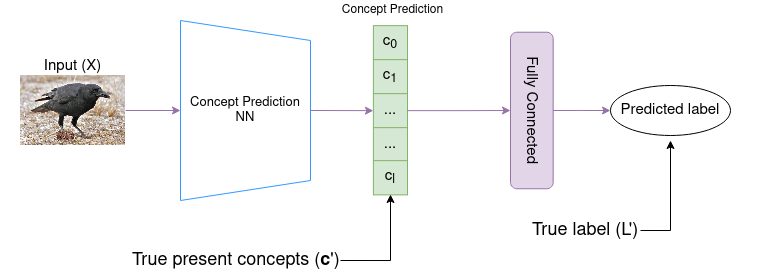
\includegraphics[width=\textwidth]{concept-bottleneck-pipeline/original-concept-bottleneck-model.png}
\label{original-concept-bottleneck}
\end{figure}

An end-to-end NN is transformed into a concept bottleneck one by forcing it to predict human-defined concepts before the final labels.
The final result of the model can then be interpreted by verifying the concepts used when making a decision.
For example, consider a bird prediction problem where human-defined concepts consist of the colour of the beak, wings and body.
If a bird is a crow, the model would predict that it has a black body, wings and beak before indicating that it is a crow.
From those results, an explanation \emph{The bird is a crow because it has black wings, black beak and black body} could be generated.

In this chapter, we take the concept bottleneck idea further.
We mine human-understandable concepts from text explanations of a label in place of a predefined set of concepts.
Such an approach would significantly simplify applying concept bottleneck pipelines in any domain.
It removes the need to predetermine an appropriate set of concepts and manually label all data points where they occur.
Text explanations, on the other hand, are sometimes readily available. For example, we could immediately use a patient's medical history report.
If the explanations are not readily available, they are easy to produce.


% Talk about Vikranth's work
\section{Inherited Work}
\label{inherited-work}

The work on the concept bottleneck pipeline has not been done from scratch.

This chapter itself is a continuation of the ideas proposed by Jeyakumar et al. in \emph{Automatic Concept Extraction for Concept Bottleneck-based Video Classification} \cite{RefWorks:RefID:16-2021automatic}. This paper failed to meet the acceptance threshold for the \href{https://iclr.cc/}{ICLR 2022} conference. 

The main contribution by Jeyakumar et al. is the \emph{Concept Discovery and Extraction Module} (CoDEx), a module that automatically uses explanations to extract text concepts.
That module has been applied to the MLB-V2E dataset, a baseball video dataset with explanations. \\
The architecture involving the \emph{Concept Discovery and Extraction Module} is shown in the figure \ref{vikranth-concept-bottleneck}. 
Generally, it is very similar to the standard architecture of the concept bottleneck architecture shown in the figure,\ref{original-concept-bottleneck} only with the CoDEx module replacing the true present concepts.

\begin{figure}[h]
\caption{Schematic representation of the concept bottleneck pipeline presented by Jeyakumar et al. (adapted from \cite{RefWorks:RefID:16-2021automatic})} 
\vspace{5pt}
\centering
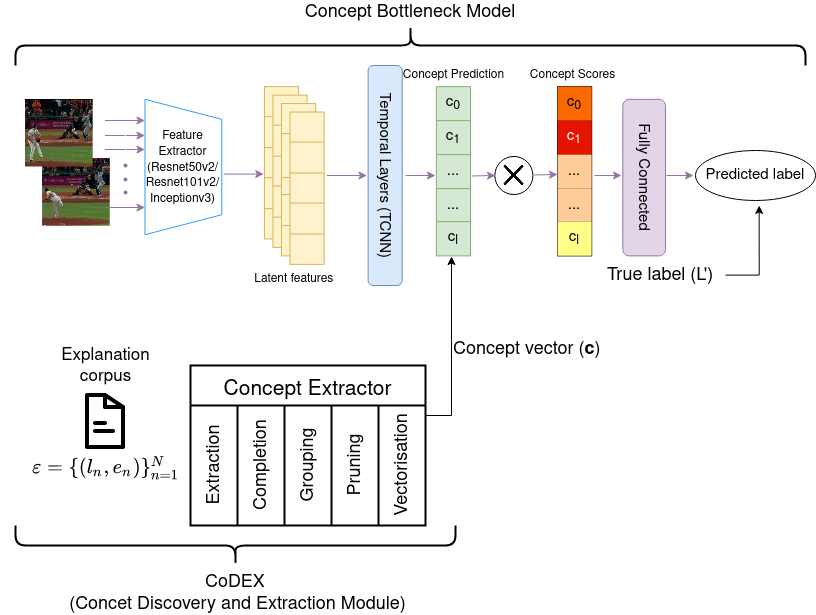
\includegraphics[width=\textwidth]{concept-bottleneck-pipeline/vikranth-concept-bottleneck.png}
\label{vikranth-concept-bottleneck}
\end{figure}


Jeyakumar et al. replace the set of human-crafted present concepts with the output of a CoDEx. 
In addition, to better understand each concept's impact on the final prediction, they add an attention layer after the concept layer to determine the concepts have more impact on the final prediction.
They extract the top three concepts with the highest attention score from that layer, which they use as explanations for a particular label. \\

\emph{Concept Discovery and Extraction Module} design is a vital element of the paper.
The CoDEx presented in the paper consists of 6 stages: \textbf{cleaning}, \textbf{extraction}, \textbf{grouping}, \textbf{completion}, \textbf{pruning}, and \textbf{vectorisation}. \\
The \textbf{cleaning} stage removes videos/explanations which are corrupted. \\
Using a constituency parser and a rule-based methodology, the \textbf{extraction} step determines if a portion of the phrase should be included as a candidate concept. 
The constituency parser uses the rules shown in the following table to extract concepts:

\begin{center}
\begin{tabular}{ |p{2cm}|p{12cm}|  }
 \hline
 \multicolumn{2}{|c|}{Rules determining whether a candidate concept should be included or excluded} \\
 \hline
 rule name & rule \\
 \hline
 Inclusion 1 & noun/pronoun → auxillary (optional) → particle (optional) → verb (optional) \\
 Inclusion 2 & noun/pronoun → auxiliary whose lemma is 'be' → any token \\
 Exclusion & subordinating conjunction \\
 
 \hline
 
\end{tabular}
\label{inclusion-exclusion-rules}
\end{center}

The \textbf{completion} stage looks up for concepts identified in some explanations while not other ones due to the behaviour of the constituency parser.
That stage is done by the substring lookup of existing concepts in all sentences. \\
The \textbf{grouping} step attempts to group concepts with similar meanings using agglomerative clustering \cite{RefWorks:RefID:13-mullner2011modern}.  \\
The \textbf{pruning} stage attempts to keep highly informative concepts by picking the smallest concept subset such that the mutual information \cite{RefWorks:RefID:30-mackay2004information} between the label and a concept vector does not fall below a certain percentage $\gamma$.
This problem is not solved precisely, but rather concepts are inserted using a greedy approach until the mutual information between the label and the newly constructed vector is not below a percentage $\gamma$. The authors chose $\gamma = 0.9$ as an appropriate value. \\
The vectorisation constructs the N x K concept matrix, where K is the number of concepts and N is the number of data points. 
The cell (n, k) is set to one if the concept k occurs for the data point n, zero otherwise.

After all these stages, a binary vector is produced for each data point, which is used in the NN training procedure.
Jeyakumar et al. train the neural network using the joint training approach, where they optimise for both the concept loss and final loss at the same time.
The concept loss is a binary cross entropy loss between a predicted concept vector and the CoDEx-produced true vector. In contrast, the final loss is a standard categorical cross entropy loss used for classification.

Using the CoDEx and the joint training procedure, the authors showed that their concept bottleneck pipeline had comparable performance to a standard end-to-end model.
In addition, the explanations they extracted were overwhelmingly better than the most common explanations.

% Changes we made to the concept bottleneck pipeline
\section{Adaptions to the Concept Bottleneck Pipeline}

In this chapter, we adapt the CoDEx part of the concept bottleneck pipeline to improve the performance and explainability of the entire model.

The \textbf{extraction} and the \textbf{completion} phase of the CoDEx have been removed from the pipeline.
The former used a rule-based approach to extract concepts.
The latter finds all concepts discovered by the constituency parser in one sentence but not in another using substring matching.

The removed stages are pretty and failed to account for a lot of information the video explanations conveyed.

To replace them extraction and completion we included \textbf{atomisation}, \textbf{generalisation} and \textbf{simple pruning} steps. \\
The chapter \ref{solving-nlp-tasks-logically} explains the first two stages (tasks) in great detail.
The \textbf{atomisation} stage splits provided sentences into one or more atomic sentences. 
Recall that the atomic sentences are sentences which an NLP expert cannot decompose into multiple valid sentences.
This procedure is done using hand-crafted interpretable rules, which are presented in the section \ref{solving-atomisation-task} along with the thought process for choosing the final solution.

The \textbf{generalisation} stage should extract all concept sentences from an atomic one. 
As explained in the section \ref{sentence-type-definitions}, the concept sentence is a syntactically correct sentence obtained by modifying a sentence's syntax tree.
To extract the concept sentences from an atomic sentence, we use a solution learned by ILASP, with the learning procedure described in \ref{solving-generalisation-task}.

The \textbf{simple pruning} stage, included between \textbf{generalisation} and \textbf{grouping} stage, is the simplest out of any of the steps present. 
It removes the concept if it fails to occur at least three times in the dataset.
The sole reason for including this stage is to speed up the subsequent steps because it slightly reduces the overall performance of the pipeline.
% INSERT reference to bird-flowers dataset DONE
CoDEx pipeline for the bird-flowers dataset \cite{RefWorks:RefID:69-wah2011caltech-ucsd} (\ref{applicability-in-other-domains}) takes less than an hour when the \textbf{simple pruning} stage is not included, which increases to over 10 hours without it.
This stage is only included when the CoDEx pipeline takes too long to compute otherwise because it is lossy.

The diagram summarising the new concept bottleneck pipeline is shown in the figure \ref{full-architecture-diagram}.

% TODO: fix X in picture, add boxes for the three parts, missing outlining X as attention module
\begin{figure}[h]
\caption{The entire pipeline for the classification of the MLB-V2E dataset using the concept bottleneck model.} 
\centering
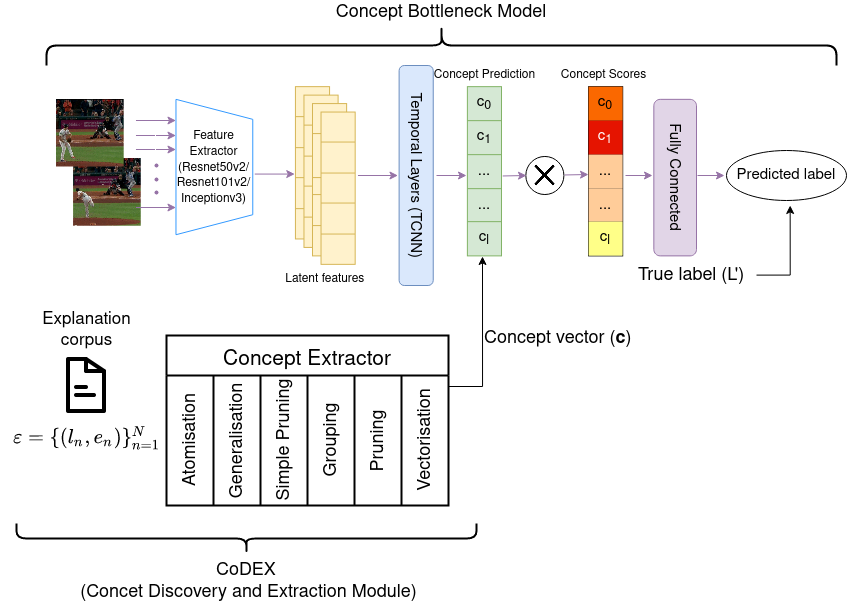
\includegraphics[width=\textwidth]{concept-bottleneck-pipeline/new-concept-bottleneck-pipeline.png}
\label{full-architecture-diagram}
\end{figure}

There were recent concerns about the joint training procedure not truly accounting for concepts in their final predictions \cite{RefWorks:RefID:68-margeloiu2021concept}. 
So, we also attempt to use the sequential training procedure, isolating the training of concept and label prediction parts of the network.
Such a training procedure performs similarly in \cite{RefWorks:RefID:35-koh2020concept}, so we expect the same.

\section{Evaluation}

This section will discuss how well the newly presented CoDEx pipeline performs.
Any results produced will be compared with the previous iteration of the concept bottleneck pipeline and the uninterpretable end-to-end model, if applicable.
To keep concept bottleneck pipelines easily comparable, we prune the concepts such that only 78 of them remain.
This number was a desirable value for the original concept bottleneck pipeline \cite{RefWorks:RefID:16-2021automatic}.

Each concept bottleneck model is also trained using both joint and sequential models, unlike the \ref{inherited-work} which only uses the joint model.
% INSERT: Cite "do concept bottleneck models work as intended" DONE
The difference between the two is that the joint optimises losses for both concepts and labels simultaneously, which sometimes overrules the nature of the concept bottleneck pipeline.
The sequential training model freezes the learned concept prediction layers, so the model must determine the final label from the concept predictions themselves \cite{RefWorks:RefID:68-margeloiu2021concept}.

For completeness, the architectures used to train the models are presented in the Appendix \ref{concept-bottleneck-architectures}.

Also, we evaluate the concept bottleneck model on a new birds-flowers dataset, which combines randomly selected images from the CUB-200-2011 \cite{RefWorks:RefID:69-wah2011caltech-ucsd} and 102 Category Flower Dataset \cite{RefWorks:RefID:70-nilsback2008automated} along with their descriptions.
This evaluation inspects how well the concept bottleneck pipeline translates to different domains.

Finally, we will critically analyse the strengths and limitations of the implemented method and suggest areas for future improvement.

\subsection{CoDEx based evaluations}

% TODO: insert tables in the appendix.
By manually observing the concepts produced (Appendix X), both methods extract relevant concepts for the problem, although not all are perfect.
For example, the new method extracts a concept \emph{It was} which is not a relevant concept.
In general, the new method seems to extract concepts which better describe the labels, but we evaluate this belief concretely in this subsection.


\subsubsection{Measuring Cumulative MI}

% INSERT ref MacKay book; maybe insert Venn diagram from Wikipedia.   DONE (not the wiki bit)
Mutual Information $I(X;Y)$ \cite{RefWorks:RefID:30-mackay2004information} is defined as $I(X; Y) \equiv H(X) - H(X|Y)$. 
It estimates the average reduction in uncertainty about $x$ caused by understanding $y$'s value or vice versa. 
It is the average quantity of information conveyed by $x$ regarding $y$.

In the context of this project, the discrete variable $Y$ is a set of label outcomes. A possible outcome is a number between 0 and 4, where each number represents an event which occurred.
The discrete variable $X$ represents a set of extracted concepts with size $k$, where $k$ is a parameter tested in this evaluation.

In addition, given that the cumulative MI is under consideration, the set of size $k$ should ideally contain $k$ \emph{maximally informative} concepts, i.e. those which will result in the highest mutual information score.
However, finding such a set is infeasible as the problem is combinatorial \cite{RefWorks:RefID:16-2021automatic}. Still, we can get a highly informative set by greedily adding a single concept that improves MI the most. 

So, by measuring cumulative MI, we can determine how good the extracted concepts are at describing the labels.

The results can be seen in the figure \ref{cummulative-mi-graphs}.

% TODO: replace this with a new version

\begin{figure}[h]
\caption{Cumulative MI graphs using old and new concept extraction pipeline}
\centering
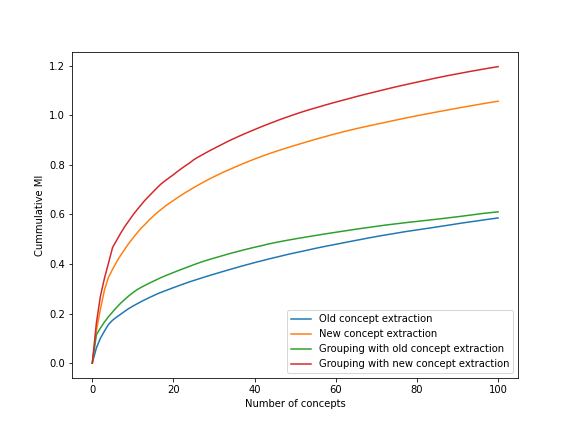
\includegraphics[width=\textwidth]{concept-bottleneck-pipeline/Cummulative MI graphs.png}
\label{cummulative-mi-graphs}
\end{figure}

% TODO: talk about specific numbers

It shows that the new concept extraction method drastically outperforms the old approach for the first 100 concepts.
Since only 78 are taken for the entire pipeline training, these results indicate that the new concept bottleneck performance should drastically improve.


\subsubsection{Concept Prediction Performance}

A corollary of the higher concept mutual information is a higher concept prediction accuracy.

Consider a classifier which would result in the highest possible accuracy for a dataset from binary vectors to labels.
Such a classifier assigns the correct label to any non-conflicting binary vector and the most common label to any conflicting binary vector. 
A conflicting vector is one whose outcome can result in multiple different labels.
The maximum possible accuracies are summarised in the table below:

\begin{center}
\begin{tabular}{ |M{3 cm}||M{3cm}|M{3cm}|  }
 \hline
 \multicolumn{3}{|c|}{Maximum accuracy comparison} \\
 \hline
 \hline
  & Old concept extraction&New concept extraction\\ 
 \hline
 Training dataset & 51.1\% & 78.6\% \\
 Test dataset & 47.7\% & 87.7\% \\
 \hline
\end{tabular}
\end{center}

The highest possible accuracy with the new concept extraction for training and the test set is much greater than the values achievable with the old procedure.

To validate these results translate into practice, we train an MLP classification model from binary vectors to labels with both old and new concept extraction.
% INSERT reference RoBERTa DONE
In addition, a RoBERTa transformer model \cite{RefWorks:RefID:84-liu2019roberta:} is trained directly from an unedited human-generated explanation to estimate how much information is lost through concept extraction.
The results are summarised in the table below:
\begin{center}
\begin{tabular}{ |M{3cm}|M{3cm}|M{3 cm}|  }
 \hline
 \multicolumn{3}{|c|}{Practical accuracy results} \\
 \hline
 \hline
 Transformer& Old Concepts & New concepts\\ 
 \hline
 0.953 $\pm$ 0.002 & 0.450 $\pm$ 0.001 & 0.820 $\pm$ 0.002 \\
 \hline
\end{tabular}
\end{center}

These experiments convince us that the performance of a concept bottleneck performance should improve.
They also suggest that there is still room for improvement for the concept extraction since there is a 19\% accuracy improvement by training a model directly from text.

\subsection{Performance of the Full Concept Bottleneck Pipeline}

The model performance is measured on the entire concept bottleneck pipeline.
We measure the final accuracy of the models with identical architectures (Appendix \ref{concept-bottleneck-architectures}) using new and old concept extraction. 
In addition, the quality of the concept prediction is also measured as it can help understand whether the concept bottleneck nature of the model is indeed considered. \\
The precision metric is used to measure the concept prediction performance because detecting a subset of present concepts is often enough to determine the final label correctly.
Furthermore, most concept values are set to 0 for any data point, so metrics considering true negatives would have a high value even when the actual concept prediction is poor.
The final label prediction is measured using accuracy, as we want the predictions to be correct most of the time.
The predictive accuracies are also compared with an end-to-end model with an identical architecture, the highest value the concept bottleneck models could achieve.

The model accuracies are presented in the below:

\begin{center}
\begin{tabular}{ |M{3cm}|M{3cm}|M{3 cm}|  }
 \hline
 \multicolumn{3}{|c|}{Final label prediction accuracy} \\
 \hline
 \hline
 No concepts& Old Concepts & New concepts\\ 
 \hline
 0.687 $\pm$ 0.005 & 0.623 $\pm$ 0.005 & 0.685 $\pm$ 0.005 \\
 \hline
\end{tabular}
\end{center}

As expected, the model without concepts has a higher mean accuracy than both concept bottleneck models. 
In addition, we expect that the new concept extraction outperforms the old one due to the higher mutual information value its concepts have. \\
However, we expected a much more significant performance difference between the concept bottleneck approaches due to a stark contrast in mutual information values and concept-only predictive accuracies.
To understand why that is the case, we need to consider the precision values of the concepts:

\begin{center}
\begin{tabular}{ |M{3cm}|M{3 cm}|  }
 \hline
 Old concepts precision & New concept precision \\ 
 \hline
 0.163 $\pm$ 0.003 & 0.172 $\pm$ 0.005 \\
 \hline
\end{tabular}
\end{center}

The concept predictions are extremely poor compared to the final results.
So, it seems that concepts serve more as proxies for holding NN final prediction information instead of genuinely being learned by the network.
This statement is backed up by the fact that old concept prediction even outperforms the prediction results directly from concepts, which would not have been possible in an actual concept bottleneck model \cite{RefWorks:RefID:68-margeloiu2021concept}.
Nevertheless, such low prediction values may not result in poor explanations since concepts could exist in the video but not in the CoDEx matrix.

To force the concept bottleneck nature of the model, we train another model using the sequential approach. 
Such an approach first trains the concept prediction part of the network before training the network from concept predictions to final labels, with the results shown in the table below.

\begin{center}
\begin{tabular}{ |M{3cm}|M{3cm}|M{3 cm}|  }
 \hline
 \multicolumn{3}{|c|}{Sequential training prediction accuracy} \\
 \hline
 \hline
 No concepts& Old Concepts & New concepts\\ 
 \hline
 0.687 $\pm$ 0.005 & 0.354 $\pm$ 0.019 & 0.579 $\pm$ 0.008 \\
 \hline
\end{tabular}
\end{center}

\begin{center}
\begin{tabular}{ |M{3cm}|M{3 cm}|  }
 \hline
 Old concepts precision & New concept precision \\ 
 \hline
 0.610 $\pm$ 0.018 & 0.479 $\pm$ 0.016 \\
 \hline
\end{tabular}
\end{center}

The sequential training has drastically improved concept precision values as the predictions from the final layer could not have overridden the concept predictions.
In addition, the sequential training has reduced the performance of both models.
It has made the difference between the results much bigger, clearly showcasing that new concept predictions are significantly better than the old ones.

However, the decrease in performance is undesirable.
If the concepts present in the video coincide with the concepts predicted by the network, joint training should be preferred as it has a higher performance.
We further quantitatively evaluate the concepts predicted by the joint network to see if they would constitute good explanations.

\subsection{Explainability of the Labels}

% INSERT appendix baseball rules quickly


The main reason we use the concept bottleneck pipeline is to allow interpretation of final labels using the intermediate concepts.
To do so, we compare the concept values after attention as human subjects prefer them over all alternatives in almost 70\% of the cases in \cite{RefWorks:RefID:16-2021automatic}.

We consider a concept as active for a data point if it has a score close to the maximum.
This behaviour was chosen because there was a sharp concept value drop of more than 50\% from the few top values, making these concepts a lot less relevant for the final decision.


Unfortunately, due to a lack of resources, we have not been able to repeat the Mechanical Turk study done in \cite{RefWorks:RefID:16-2021automatic}. 
Instead, we only discuss three randomly selected test examples and qualitatively compare the old and new concept predictions for them: \\


% Label 1: curr_point = 78, id: KP4EFXZPM12B
Sourced explanation 1: \emph{The batter swung the bat and hit it into foul territory. This was called a foul ball by the ump}. \\
True label 1: foul.

The results are shown in \ref{concepts-results-1}.
The video consisted of a batter hitting the ball in the air behind him in the foul territory.
Both networks accurately predict this sequence as a foul.

\begin{figure}[h]
\caption{Most relevant concepts for example 1, along with their concept scores. The LHS shows the ones predicted by the old concept bottleneck, while the RHS is predicted by the new one.}
\centering
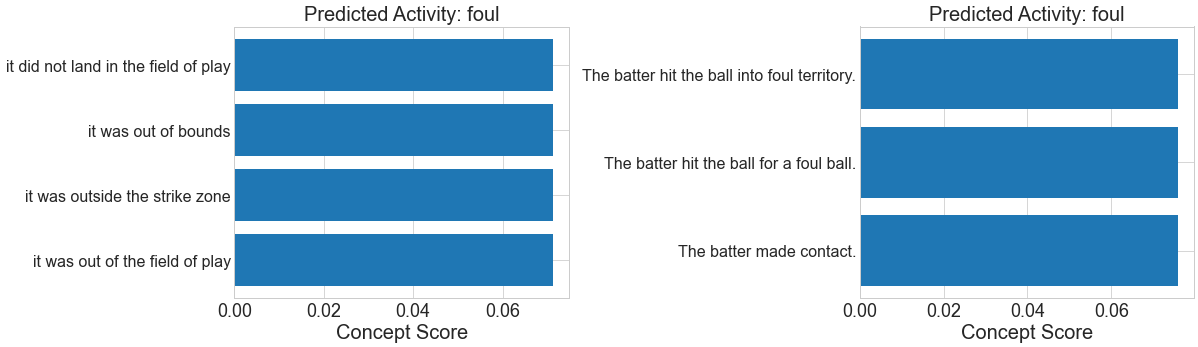
\includegraphics[width=\textwidth]{concept-bottleneck-pipeline/explanations_concepts1.png}
\label{concepts-results-1}
\end{figure}

For the new concept bottleneck network, all predicted concepts are correct.
The batter has indeed made contact; the ball went into the foul territory and was undoubtedly a foul ball.
They describe well all the events that happened.
On the other hand, old concepts also perform well in this case.
One should be able to determine that the final label should be foul from the concepts. 
The concept \emph{it was outside of strike zone} is wrong. 
If that piece of information is indeed correct, the true label would have been \emph{ball} instead of the \emph{foul}.
In addition, \emph{it was out of bounds}, \emph{it did not land in the field of play}, \emph{it was out of field of play} all capture that the ball landed outside of the allowed territory.
It may be sufficient only to present one such concept.

Although both concepts are good enough to predict the final label accurately, a human subject would usually prefer the new one.
It is not only because the old concept bottleneck presents an incorrect sentence but also because the new concepts seem much clearer.
The user does not need to infer what "it" is referring to. \\

% Label 2: curr_point = 122, id: SAGXX461QCAB
Sourced explanation 2: \emph{The batter hit it in play and it was not caught.} \\
True label 2: play

\begin{figure}[h]
\caption{Most relevant concepts for example 2, along with their concept scores. The LHS shows the ones predicted by the old concept bottleneck, while the RHS is predicted by the new one.}
\centering
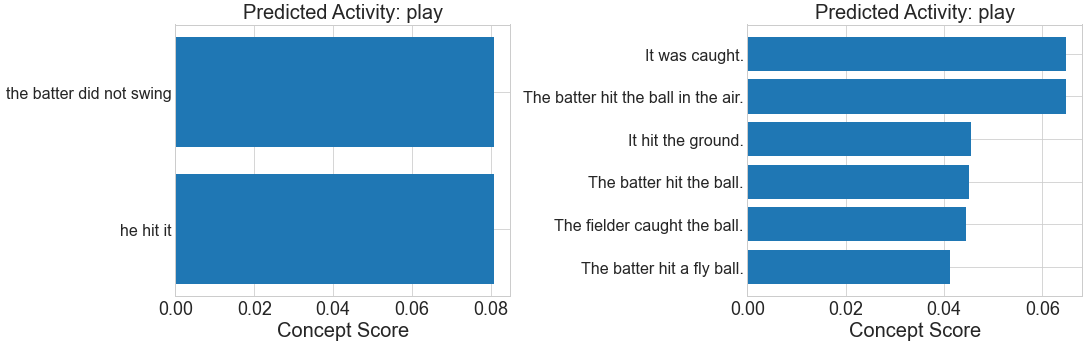
\includegraphics[width=\textwidth]{concept-bottleneck-pipeline/expalantions_concepts2.png}
\label{concepts-results-2}
\end{figure}

The results are shown in \ref{concepts-results-2}.
The video in explanation 2 showed a batter hitting a fly ball which an outfielder caught after it hit the ground.
Both networks accurately predict this sequence as a play.

Unlike the previous video, a baseball expert would not determine the final label from both explanations.
The old concept prediction only predicted two conflicting concepts, out of which only \emph{he hit it} is correct.

On the contrary, the new concept extraction predicted all relevant events that have occurred in the video.
These concepts have some redundancy, such as \emph{It was caught} and \emph{The fielder caught the ball} presenting the same thing.
Moreover, the new concepts showcase a finer level of granularity in event prediction by predicting that a fly ball has occurred. 
The concept scores might slightly confuse a user, in this case, as they highlight two concepts more than the others. 
If these were showcased on their own, they would seem more related to \textit{out} rather \emph{play}. \\

% Label 3: curr_point = 201, id: ZLP8NFBVSNHS, strike
Sourced explanation 3: \emph{the batter did not swing at a ball in the strike zone}. \\
True label 3: strike

The results are shown in \ref{concept-results-3}.
Both networks correctly predict this sequence as a strike.

\begin{figure}[h]
\caption{Most relevant concepts for example 3, along with their concept scores. The LHS shows the ones predicted by the old concept bottleneck, while the RHS is predicted by the new one.}
\centering
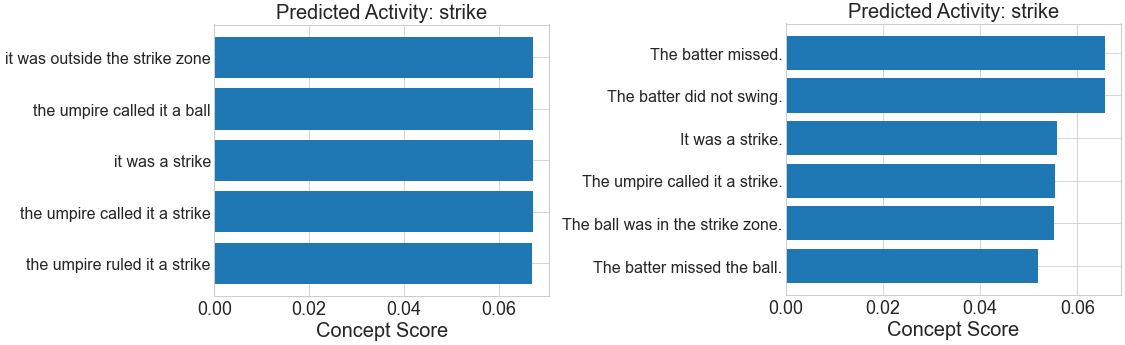
\includegraphics[width=\textwidth]{concept-bottleneck-pipeline/explanations_concepts3.png}
\label{concept-results-3}
\end{figure}

Again, the new concept extraction pipeline seemed to have extracted better concepts for describing the label.
There are two reasons for it: they are more accurate and describe multiple events from which the final label could be inferred.

The old concept prediction pipeline predicted two incorrect concepts: \emph{it was outside of the strike zone} and \emph{the umpire called it a ball}.
All of the newly inferred concepts are correct, on the contrary.

The new concept prediction describes multiple relevant events. 
For example, it describes both the umpire ruling the event as a strike and the ball being in the strike zone.
On the other hand, only the umpire calling the pitch a strike was predicted. 
The other two concepts either describe the same thing \emph{the umpire ruled it a strike} or have predicted the final label instead of a concept \emph{it was a strike}.
Note that the latter was also predicted in the new concept bottleneck pipeline. 
That sentence should be omitted since it would be a meaningful statement in any explanation describing why the label occurred. \\

To sum up, there seems to promise that the new method improves explanations in both accuracy and the level of detail.
We should create a human study in the future to validate these claims.

In addition, notice that the model should not predict a few of the concepts chosen if CoDEx output was used as the ground truth.
However, they were mostly correct, especially for the new concept extraction.
So, the poor precision value may not necessarily hurt explanations, but rather correct concepts may not often be captured by the CoDEx module.
These results may even suggest that joint network training helps extract a good set of concepts by using the final label information. 


\subsection{Applicability in other Domains}
\label{applicability-in-other-domains}

% TODO: finish

As argued, the idea presented in this section, in theory, is not tied to video applications.
This evaluation measures how well the CoDEx module fares when applied to a birds-flowers dataset.
This dataset consists of 2000 birds/flowers images taken from \cite{RefWorks:RefID:87-wah2011caltech-ucsd} and \cite{RefWorks:RefID:70-nilsback2008automated}, combined with image descriptions generated for these respective datasets.
As such, the explanations are written to describe the image rather than its relevance to the label.
It was chosen due to its simplicity for a standard NN, as demonstrated by the high accuracy of a non-concept bottleneck model. 
In addition, the explanations were also readily available to use for concept prediction.

% INSERT Appendix X
By observing the concepts extracted, we see that the set of concepts may be applicable. 
For example, the CoDEx extracts the following concepts together with their occurrence in the dataset:
\begin{verbatim}
The bird has feathers. % 18
This flower has pistil. % 18
\end{verbatim}
Despite the sentence structure immediately highlighting whether it is a bird or a flower, the model would nevertheless try to learn what are feathers and pistils.
The issue is the count occurrence for doing so.
More than 18 birds in the dataset have feathers, and more than 18 flowers have pistils.
This poor count results from label explanations extracted from the two label descriptions focusing on differences between different species of birds/flowers instead of the differences between the two.
In addition, not all concepts are helpful, such as \emph{This bird has}, but in general, there seems to be enough information to determine the final labels correctly.

On the other hand, the concepts produced by the old approach seem much worse. 
It is often quite unclear which label they correspond to, such as \emph{that are oval shaped}.
Or, there are a few very specific concepts grouped with other similarly long concepts. 
For example, a concept \emph{this is a white and black bird with a black crown and a long black beak} would fall into that category.

The dominant (most frequent) extracted concepts are included in Appendix X, along with the frequency of the group occurrence.

To validate whether the initial observations translate to tangible results, we evaluate how well can an MLP predict the final label.
The input are the concept prediction vectors produced by old and new CoDEx modules.
The results are compared against a fine-tuned RoBERTa transformer \cite{RefWorks:RefID:84-liu2019roberta:} trained directly from text to estimate how much information is lost by mining concepts.

\begin{center}
\begin{tabular}{ |M{4cm}||M{3cm}|M{3cm}|M{3cm}|  }
 \hline
 \multicolumn{4}{|c|}{Results from explanations only} \\
 \hline
 & Transformer & Old concepts & New concepts \\
 \hline
 Final accuracy & 1.000 $\pm$ 0.000 & 0.844 $\pm$ 0.008 & 0.874 $\pm$ 0.006 \\
 \hline
\end{tabular}
\end{center}

The newly extracted concepts can better distinguish between labels, although the difference is not as big as for the baseball dataset.
The main reason for a loss in accuracy is the case where all inputs are 0, where any concept that was detected ended up being pruned.
This case happens more often for the old concept extraction, but the new one is not immune.
As the transformer has perfect accuracy, it is clear that it is straightforward to distinguish between the two labels from descriptions.

We further evaluate the jointly trained models with identical architecture (Appendix \ref{concept-bottleneck-architectures})and hyper-parameters using old, new or no concepts in the intermediate layers:

\begin{center}
\begin{tabular}{ |M{4cm}||M{3cm}|M{3cm}|M{3cm}|  }
 \hline
 \multicolumn{4}{|c|}{Full model results} \\
 \hline
 & No concepts & Old concepts & New concepts \\
 \hline
 Final accuracy & 0.979 $\pm$ 0.004 & 0.987 $\pm$ 0.002 & 0.989 $\pm$ 0.002 \\
 Concept precision & / & 0.367 $\pm$ 0.021 & 0.212 $\pm$ 0.009 \\
 \hline
\end{tabular}
\end{center}

The final accuracies of the models all have similarly high values, which is desirable.
However, the concept precision results are similarly poor as the results for the MLB-V2E \cite{RefWorks:RefID:16-2021automatic} dataset.
As mentioned, the text explanations do not describe all features that a bird/flower has.
For that reason, the CoDEx pipelines often fail to account for many concepts present in the image but not the explanations during training.
In addition, the reason behind higher concept accuracy may be related to the NN optimising for a positive concept value much more often with new concept extraction.
The training set for the new concept bottleneck pipeline has more than twice the number of detected concepts.

We further present the predicted concept values for randomly selected data points shown in the figure \ref{bird-concept-predictions} and \ref{flower-concept-predictions}.

\begin{figure}[h]
\caption{The most relevant concepts for the image are shown below, along with their concept scores. The LHS shows the ones predicted by the old concept bottleneck, while the RHS is predicted by the new one.}
\centering
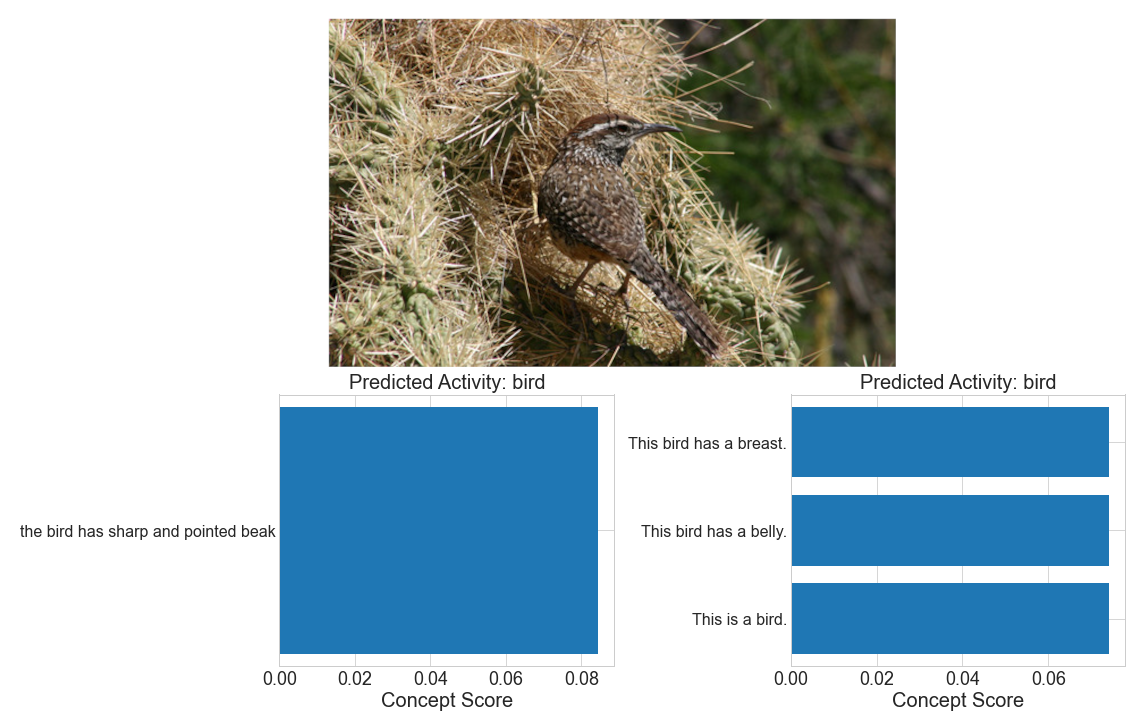
\includegraphics[width=\textwidth]{concept-bottleneck-pipeline/birds_predictions.png}
\label{bird-concept-predictions}
\end{figure}

For the bird example in \ref{bird-concept-predictions}, both outcomes could be better.
The old concept bottleneck pipeline only shows a true but very specific feature.
On the other hand, the new concept bottleneck pipeline predicted better concepts that would describe some birds well.
However, given the bird's orientation in the image, specifying that it has a breast and belly seems counter-intuitive.

\begin{figure}[h]
\caption{The most relevant concepts for the image are shown below, along with their concept scores. The LHS shows the ones predicted by the old concept bottleneck, while the RHS is predicted by the new one.}
\centering
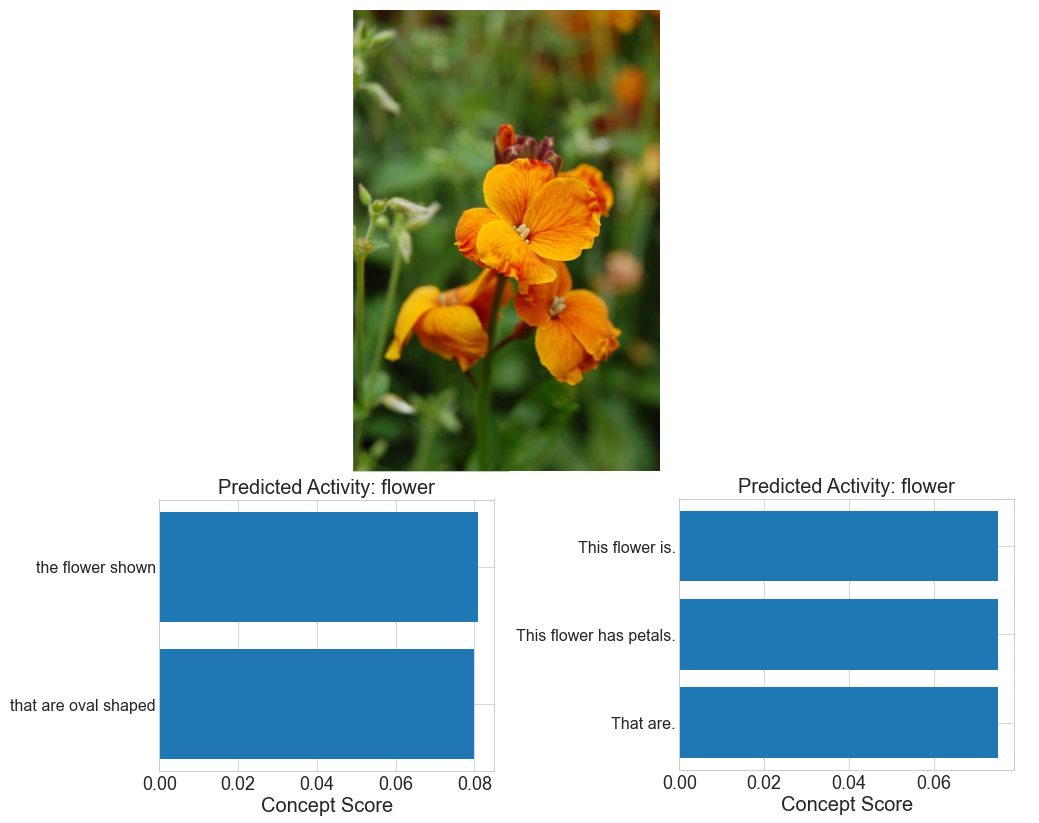
\includegraphics[width=\textwidth]{concept-bottleneck-pipeline/flower_predictions.png}
\label{flower-concept-predictions}
\end{figure}

The results for the example in \ref{flower-concept-predictions} could be better.
The new concept bottleneck extracts well that \emph{this flower has petals}.
However, the other two concepts are not even valid sentences.
The old concept bottleneck similarly extracts concept texts missing crucial information.


To sum up, neither method extracts good concepts for the bird-flowers dataset.
The conjunction of bird/flower image descriptions did not prove sufficient information to extract good concepts for the final explanation.
We believe that for the method to work, the explanations need to be generated to highlight why this data point should be assigned precisely to some class and not the other.


\subsection{Discussion}

In this chapter, we show that the addition of atomisation and generalisation greatly helps the concept bottleneck pipeline performance.
When incorporated into the concept bottleneck pipeline, the new CoDEx has much higher mutual information,  predictive accuracy, and performance.
In addition, there is an indication that its explanation generation is much better.

We also highlight a possible issue with joint training of a concept bottleneck model that may not truly consider the concept bottleneck nature of the problem.
However, to achieve comparable performance with the sequential training, we need to find a way to capture all the concepts that occur in the video.

Further improvements of the concept bottleneck CoDEx should incorporate a mechanism for detecting concepts detected in the video/image, but not the explanation.
With such a mechanism, training the concept prediction part of the network would yield a much better performance, which should improve the accuracy of generated explanations.

Although the birds/flowers experiment failed to extract good explanations for images, it demonstrated that the method presented in this chapter applies to data of different modalities, not just videos.
The experiment required no change of the CoDEx pipeline to mine concepts from image explanations.
